% =============================================================================
% CTM: Conv-Temporal-Mamba Architecture for Stock Prediction
% Comprehensive Architecture Guide
% =============================================================================
\documentclass[11pt,a4paper]{article}

% ── Packages ──
\usepackage[utf8]{inputenc}
\usepackage{amsmath,amssymb,amsthm}
\usepackage{mathtools}
\usepackage{bm}
\usepackage{booktabs}
\usepackage{geometry}
\usepackage{hyperref}
\usepackage{enumitem}
\usepackage{algorithm}
\usepackage{algorithmic}
\usepackage{listings}
\usepackage{xcolor}
\usepackage{tikz}
\usepackage{caption}
\usepackage{subcaption}
\usepackage{array}

\geometry{margin=2.5cm}
\hypersetup{colorlinks=true,linkcolor=blue,citecolor=blue,urlcolor=blue}

% ── Notation ──
\newcommand{\R}{\mathbb{R}}
\newcommand{\E}{\mathbb{E}}
\newcommand{\Var}{\operatorname{Var}}
\newcommand{\Cov}{\operatorname{Cov}}
\newcommand{\softplus}{\operatorname{softplus}}
\newcommand{\softmax}{\operatorname{softmax}}
\newcommand{\SiLU}{\operatorname{SiLU}}
\newcommand{\sigmoid}{\sigma}
\newcommand{\diag}{\operatorname{diag}}
\newcommand{\loss}{\mathcal{L}}
\newcommand{\ind}{\mathbbm{1}}
\newcommand{\norm}[1]{\left\|#1\right\|}
\newcommand{\abs}[1]{\left|#1\right|}
\newcommand{\bA}{\bm{A}}
\newcommand{\bB}{\bm{B}}
\newcommand{\bC}{\bm{C}}
\newcommand{\bD}{\bm{D}}
\newcommand{\bx}{\bm{x}}
\newcommand{\bh}{\bm{h}}
\newcommand{\by}{\bm{y}}
\newcommand{\bW}{\bm{W}}
\newcommand{\bz}{\bm{z}}

\title{\textbf{CTM: Conv-Temporal-Mamba Architecture} \\[4pt]
       \large A Comprehensive Guide for Stock Prediction Systems}
\author{Quantitative Research}
\date{\today}

\begin{document}

\maketitle
\thispagestyle{empty}
\newpage

\tableofcontents
\newpage

%=============================================================================
\section{Executive Summary}
%=============================================================================

The Conv-Temporal-Mamba (CTM) architecture combines the \textbf{selective state
space model} (Mamba) with \textbf{causal convolutional processing} and
\textbf{temporal feature engineering} for stock return prediction. Unlike
Transformer-based approaches that scale quadratically with sequence length,
CTM achieves linear $\mathcal{O}(T)$ complexity while matching or exceeding
prediction accuracy.

This guide provides:
\begin{itemize}[nosep]
  \item A complete mathematical specification of the CTM architecture
  \item PyTorch implementation patterns derived from state-of-the-art research
  \item Quantitative loss functions optimized for trading metrics
  \item Scaling strategies from single-stock to multi-asset portfolios
  \item Verification and production deployment guidelines
\end{itemize}

\noindent\textbf{Key references:}
\begin{itemize}[nosep]
  \item Mamba: \textit{Linear-Time Sequence Modeling with Selective State Spaces} (Gu \& Dao, 2023)
  \item MambaStock: \textit{Selective State Space Model for Stock Prediction} (Shi, 2024)
  \item S-Mamba: \textit{Is Mamba Effective for Time Series Forecasting?} (Wang et al., 2025)
  \item SAMBA: \textit{Mamba Meets Financial Markets via Graph Convolution} (Mehrabian et al., 2025)
  \item DMamba: \textit{Decomposition-enhanced Mamba for Time Series} (Chen \& Sun, 2026)
  \item Mamba-ProbTSF: \textit{Uncertainty Quantification in SSM Forecasts} (Pessoa et al., 2025)
\end{itemize}

%=============================================================================
\section{Motivation: Why Mamba for Stock Prediction?}
%=============================================================================

Time series forecasting is the backbone of quantitative finance. Table~\ref{tab:comparison}
compares the three dominant sequence modeling paradigms.

\begin{table}[h]
\centering
\caption{Architecture comparison for financial time series}
\label{tab:comparison}
\begin{tabular}{lccc}
\toprule
Property & LSTM & Transformer & \textbf{Mamba (SSM)} \\
\midrule
Train complexity & $\mathcal{O}(T)$ & $\mathcal{O}(T^2)$ & $\mathcal{O}(T)$ \\
Inference per step & $\mathcal{O}(1)$ & $\mathcal{O}(T)$ & $\mathcal{O}(1)$ \\
Long-range memory & Poor & Excellent & Excellent \\
Parallel training & Sequential & Full & Full (associative scan) \\
Gradient stability & Moderate & Good & \textbf{Excellent} (diag. $A$) \\
Financial SOTA & Baseline & Strong & \textbf{New SOTA} \\
\bottomrule
\end{tabular}
\end{table}

\subsection{The Selective SSM Advantage}

The core innovation of Mamba is the \textbf{selective scan} mechanism (S6).
Standard SSMs (\texttt{S4}, \texttt{S4D}) have input-\textit{independent}
transition matrices. Mamba makes $\Delta_t$, $\mathbf{B}_t$, and $\mathbf{C}_t$
functions of the input $\mathbf{x}_t$, enabling \textit{content-based
selection}.

\textbf{Bi-Mamba Safety Note:} All Bi-Mamba processing operates exclusively on the historical lookback window $\{\mathbf{x}_{t-T+1}, \ldots, \mathbf{x}_t\}$ where $\mathbf{x}_t$ is the most recent \emph{observed} data point. No future data beyond the input window is accessed. See Section~5.3 for streaming inference implications.

The financial intuition is direct:
\begin{description}
  \item[$\Delta_t$ (step size)] Controls adaptation speed. Large $\Delta$ during
    news events (rapid regime change); small $\Delta$ during calm periods (smooth filtering).
  \item[$\mathbf{B}_t$ (input gate)] Selects which market signals enter the
    latent state. Suppresses noise during low-volatility regimes; amplifies predictive
    signals at turning points.
  \item[$\mathbf{C}_t$ (output gate)] Controls which parts of the learned market
    state are read for prediction. The model can learn trend-following components
    in bull markets and mean-reversion in range-bound markets.
  \item[$\overline{\mathbf{A}}_t = \exp(\Delta_t \odot \mathbf{A})$ (state decay)]
    The ``memory half-life.'' Near~1 means long memory (trend regime); near~0 means
    short memory (mean-reversion).
\end{description}

\subsection{Empirical Evidence}

Recent studies consistently show Mamba-based models outperforming LSTM and
Transformer baselines on financial data:

\begin{table}[h]
\centering
\caption{Financial Mamba empirical results}
\label{tab:results}
\begin{tabular}{lccc}
\toprule
Paper & Data & Best Model & vs.\ Best Baseline \\
\midrule
MambaStock (2024) & 4 Chinese A-shares & Mamba (2-layer) & MAE~$-$18\% \\
CryptoMamba (2025) & Bitcoin multi-regime & Bi-Mamba & RMSE~$-$22\% \\
SAMBA (2025) & US equities (82 feat.) & Graph+Mamba & exceeds SOTA \\
CrossMamba (2026) & S\&P~500 & Mamba-Aug.~Trans. & $R^2 = 0.963$ \\
\bottomrule
\end{tabular}
\end{table}

%=============================================================================
\section{CTM Architecture Overview}
%=============================================================================

The CTM architecture extends vanilla Mamba with three enhancements:

\begin{enumerate}
  \item \textbf{Conv:} Causal 1D convolution captures local temporal patterns
    before the SSM, serving as a learned feature preprocessor.
  \item \textbf{Temporal:} Multi-scale temporal decomposition separates trend
    and seasonal components for specialized processing.
  \item \textbf{Mamba:} Selective SSM backbone provides linear-complexity
    long-range sequence modeling.
\end{enumerate}

\begin{figure}[h]
\centering
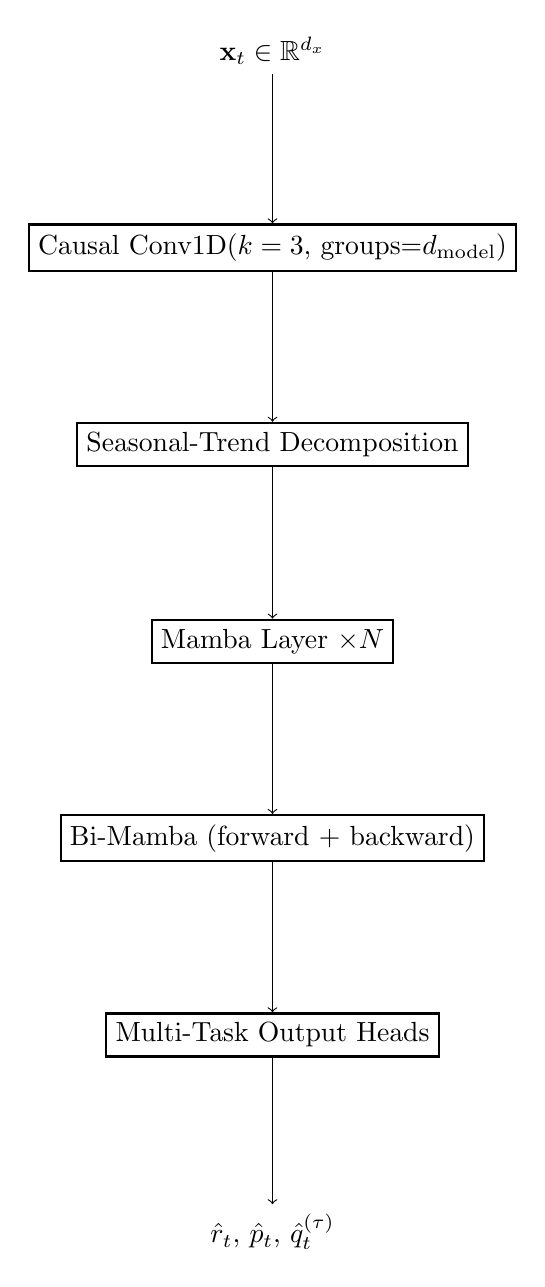
\begin{tikzpicture}[node distance=2.5cm,auto]
  % Input
  \node (input) {$\mathbf{x}_t \in \R^{d_x}$};
  % Conv block
  \node (conv) [below of=input,draw,thick,minimum width=3cm] {Causal Conv1D \\ ($k=3$, groups=$d_{\text{model}}$)};
  % Decomp
  \node (decomp) [below of=conv,draw,thick,minimum width=3cm] {Seasonal-Trend Decomposition};
  % Mamba blocks
  \node (mamba1) [below of=decomp,draw,thick,minimum width=3cm] {Mamba Layer $\times N$};
  % Bidirectional
  \node (bi) [below of=mamba1,draw,thick,minimum width=3cm] {Bi-Mamba (forward + backward)};
  % Heads
  \node (heads) [below of=bi,draw,thick,minimum width=3cm] {Multi-Task Output Heads};
  % Output
  \node (out) [below of=heads] {$\hat{r}_t$, $\hat{p}_t$, $\hat{q}_t^{(\tau)}$};
  % arrows
  \draw[->] (input) -- (conv);
  \draw[->] (conv) -- (decomp);
  \draw[->] (decomp) -- (mamba1);
  \draw[->] (mamba1) -- (bi);
  \draw[->] (bi) -- (heads);
  \draw[->] (heads) -- (out);
\end{tikzpicture}
\caption{CTM architecture overview}
\label{fig:arch}
\end{figure}

\subsection{Architecture Variants}

Based on our research, we identify five validated architecture patterns:

\paragraph{Pattern 1: Vanilla Mamba Stack (MambaStock baseline)}
2--4 Mamba layers with residual connections. Uses only selective scan with
SiLU gating. This is the simplest proven configuration for stock prediction.

\paragraph{Pattern 2: Decomposition + Specialized Modules (DMamba)}
\[
\text{Input} \to \text{Seasonal-Trend Decomp} \to
\begin{cases}
\text{Seasonal: Mamba (high-dim)}, \\
\text{Trend: MLP (low-dim)}
\end{cases} \to \text{Fuse} \to \text{Predict}
\]

\paragraph{Pattern 3: Bidirectional Mamba (S-Mamba, SAMBA)}
Processes both forward and backward passes through separate Mamba stacks,
then concatenates features before the prediction head.

\paragraph{Pattern 4: Graph + Mamba (SAMBA)}
For multi-stock prediction, adds a Chebyshev graph convolution layer after
Mamba to model inter-stock correlations with a learned adjacency matrix.

\paragraph{Pattern 5: Hybrid Mamba-Transformer (CrossMamba)}
Interleaves Mamba and attention layers, where Mamba handles long-range
dependencies and attention focuses on local patterns.

%=============================================================================
\section{Mamba Core: Selective State Space Model}
%=============================================================================

\subsection{Mathematical Formulation}

A continuous state space model maps an input signal $\mathbf{x}(t) \in \R$ to
an output $\mathbf{y}(t) \in \R$ through a latent state $\mathbf{h}(t) \in \R^N$:
\begin{align}
  \mathbf{h}'(t) &= \mathbf{A} \mathbf{h}(t) + \mathbf{B} \mathbf{x}(t) \\
  \mathbf{y}(t)  &= \mathbf{C} \mathbf{h}(t) + \mathbf{D} \mathbf{x}(t)
\end{align}
where $\mathbf{A} \in \R^{N \times N}$ is the state transition matrix,
$\mathbf{B} \in \R^{N \times 1}$ the input matrix, $\mathbf{C} \in \R^{1 \times N}$
the output matrix, and $\mathbf{D} \in \R$ the skip connection.

For discrete sequences $\{\mathbf{x}_1, \ldots, \mathbf{x}_T\}$ with step size
$\Delta$, the zero-order hold (ZOH) discretization gives:
\begin{align}
  \overline{\mathbf{A}} &= \exp(\Delta \mathbf{A}) \\
  \overline{\mathbf{B}} &= \mathbf{A}^{-1}(\exp(\Delta\mathbf{A}) - \mathbf{I}) \cdot \mathbf{B} \approx \Delta \mathbf{B}
\end{align}
where {\footnotesize $\mathbf{A}^{-1}(\exp(\Delta\mathbf{A}) - \mathbf{I})\mathbf{B}$}
is the exact ZOH and $\Delta\mathbf{B}$ is the Euler approximation (which Mamba
uses in practice for efficiency).
The discrete recurrence is:
\begin{align}
  \mathbf{h}_t &= \overline{\mathbf{A}} \mathbf{h}_{t-1} + \overline{\mathbf{B}} \mathbf{x}_t \\
  \mathbf{y}_t &= \mathbf{C} \mathbf{h}_t + \mathbf{D} \mathbf{x}_t
\end{align}

\subsection{Selective Scan (S6)}

Mamba makes $\Delta_t$, $\mathbf{B}_t$, and $\mathbf{C}_t$ functions of the
input $\mathbf{x}_t$. Given projection weights $\mathbf{W}_\Delta$,
$\mathbf{W}_B$, $\mathbf{W}_C$:

\begin{align}
  \Delta_t &= \operatorname{clamp}\bigl(\softplus(\mathbf{W}_\Delta \mathbf{x}'_{\text{conv},t} + \mathbf{b}_\Delta),\; 10^{-5},\; 20.0\bigr) \\
  \mathbf{B}_t &= \mathbf{W}_B \mathbf{x}'_{\text{conv},t} \\
  \mathbf{C}_t &= \mathbf{W}_C \mathbf{x}'_{\text{conv},t}
\end{align}

The discretization with diagonal $\mathbf{A}$ (for efficiency,
$\mathbf{A} = \diag(a_1, \ldots, a_{d_{\text{model}}})$) becomes element-wise:
\begin{align}
  \overline{\mathbf{A}}_t &= \exp\left(\Delta_t \odot \mathbf{A}\right) \\
  \overline{\mathbf{B}}_t &= \Delta_t \otimes \mathbf{B}_t^\top \quad\text{(outer product: $\overline{B}_t[c,s] = \Delta_t[c] \cdot B_t[s]$)} \label{eq:bbar}
\end{align}

The selective scan recurrence per channel $i$:
\begin{align}
  h_t[i] &= \overline{A}_t[i] \cdot h_{t-1}[i] + \overline{\mathbf{B}}_t[i,:] \cdot x'_{\text{conv},t}[i] \\
  y_{\text{ssm},t}[i] &= \mathbf{C}_t^\top h_t[i] + D[i] \cdot x'_{\text{conv},t}[i]
\end{align}

\subsection{Matrix Implementation}

In practice, all channels are processed simultaneously using batched operations:
\begin{align}
  \mathbf{h}_t &= \overline{\mathbf{A}}_t \odot \mathbf{h}_{t-1} + \overline{\mathbf{B}}_t \odot \mathbf{x}'_{\text{conv},t} \quad (\text{broadcast}) \\
  \mathbf{y}_{\text{ssm},t} &= \mathbf{C}_t^\top \mathbf{h}_t + \mathbf{D} \odot \mathbf{x}'_{\text{conv},t}
\end{align}
where $\mathbf{h}_t \in \R^{d_{\text{model}} \times d_{\text{state}}}$,
$\overline{\mathbf{A}}_t \in \R^{d_{\text{model}} \times 1}$,
$\overline{\mathbf{B}}_t \in \R^{d_{\text{model}} \times d_{\text{state}}}$.

\subsection{Full Mamba Block Forward Pass}

\begin{algorithm}[h]
\caption{Mamba block forward pass (per time step $t$)}
\begin{algorithmic}[1]
\STATE $\mathbf{z} \gets \mathbf{W}_{\text{in}} \mathbf{x}_t$ \COMMENT{Input projection: $(2d_{\text{model}}) \times 1$}
\STATE $\mathbf{z}_1, \mathbf{z}_2 \gets \text{split}(\mathbf{z})$ \COMMENT{SSM branch, gate branch}
\STATE $\mathbf{x}'_{\text{conv},t} \gets \text{causal\_conv1d}(\mathbf{z}_1)$ \COMMENT{Local feature extraction}
\STATE $\mathbf{x}'_{\text{conv},t} \gets \SiLU(\mathbf{x}'_{\text{conv},t})$ \COMMENT{Activation}
\STATE $\Delta_t \gets \operatorname{clamp}\bigl(\softplus(\mathbf{W}_\Delta \mathbf{x}'_{\text{conv},t} + \mathbf{b}_\Delta),\; 10^{-5},\; 20.0\bigr)$ \COMMENT{Step size}
\STATE $\mathbf{B}_t \gets \mathbf{W}_B \mathbf{x}'_{\text{conv},t}$ \COMMENT{Input matrix}
\STATE $\mathbf{C}_t \gets \mathbf{W}_C \mathbf{x}'_{\text{conv},t}$ \COMMENT{Output matrix}
\STATE $\overline{\mathbf{A}}_t \gets \exp(\Delta_t \odot \mathbf{A})$ \COMMENT{Discretize $\mathbf{A}$}
\STATE $\overline{\mathbf{B}}_t \gets \Delta_t \odot \mathbf{B}_t^\top$ \COMMENT{Discretize $\mathbf{B}$}
\STATE $\mathbf{h}_t \gets \overline{\mathbf{A}}_t \odot \mathbf{h}_{t-1} + \overline{\mathbf{B}}_t \odot \mathbf{x}'_{\text{conv},t}$ \COMMENT{SSM recurrence}
\STATE $\mathbf{y}_{\text{ssm},t} \gets \mathbf{C}_t^\top \mathbf{h}_t + \mathbf{D} \odot \mathbf{x}'_{\text{conv},t}$ \COMMENT{SSM output}
\STATE $\mathbf{y}_t \gets \SiLU(\mathbf{z}_2) \odot \mathbf{y}_{\text{ssm},t}$ \COMMENT{Gating}
\STATE $\mathbf{\hat{r}}_t \gets \mathbf{W}_{\text{out}} \mathbf{y}_t$ \COMMENT{Output projection}
\STATE \RETURN $\mathbf{\hat{r}}_t, \mathbf{h}_t$
\end{algorithmic}
\end{algorithm}

\subsection{Parallel Scan for Training}

The recurrence $\mathbf{h}_t = \overline{\mathbf{A}}_t \odot \mathbf{h}_{t-1} + \overline{\mathbf{B}}_t \odot \mathbf{x}'_{\text{conv},t}$
is an \textbf{associative operation} and can be computed in parallel using a
scan algorithm:

\begin{algorithm}[h]
\caption{Parallel associative scan (Blelloch, 1990)}
\begin{algorithmic}[1]
\REQUIRE Elements $\{e_t = (\overline{\mathbf{A}}_t, \overline{\mathbf{B}}_t \odot \mathbf{x}'_{\text{conv},t})\}_{t=1}^T$
\ENSURE Prefix products $\{\mathbf{h}_t\}_{t=1}^T$
\STATE \COMMENT{Phase 1: Up-sweep (tree reduction)}
\FOR{$d = 1$ to $\log_2 T$}
  \FOR{$k = 0$ to $T-1$ step $2^d$}
    \STATE $e_{k+2^d-1} \gets e_{k+2^{d-1}-1} \circ e_{k+2^d-1}$
  \ENDFOR
\ENDFOR
\STATE \COMMENT{Phase 2: Down-sweep}
\STATE $e_{T-1} \gets \text{identity}$ \COMMENT{Replace last with identity}
\FOR{$d = \log_2 T - 1$ down to $0$}
  \FOR{$k = 0$ to $T-1$ step $2^{d+1}$}
    \STATE $\text{temp} \gets e_{k+2^d-1}$
    \STATE $e_{k+2^d-1} \gets e_{k+2^{d+1}-1} \circ \text{temp}$
    \STATE $e_{k+2^{d+1}-1} \gets \text{temp} \circ e_{k+2^{d+1}-1}$
  \ENDFOR
\ENDFOR
\STATE \RETURN $\{\mathbf{h}_k\}$ extracted from $e_k$
\end{algorithmic}
\end{algorithm}

The associative operator $\circ$ is defined as:
\[
(a, b) \circ (a', b') = (a' \cdot a,\; a' \cdot b + b')
\]
which corresponds to composing two steps of the recurrence. This reduces the
sequential $\mathcal{O}(T)$ computation to $\mathcal{O}(\log T)$ parallel steps.

\subsection{Mamba-2: State Space Duality (SSD)}

Mamba-2 (Dao \& Gu, 2024) reformulates the SSM using SSD, proving that SSMs
and attention are mathematically dual. Key improvements:

\begin{itemize}
  \item \textbf{Larger state dimension:} $d_{\text{state}} = 64$--$128$ (vs.\ 16 in Mamba-1)
  \item \textbf{Scalar-times-identity A matrix:} Simplified from full diagonal
  \item \textbf{Chunked matmul:} Divides sequence into chunks; 80--90\% tensor core utilization
  \item \textbf{Single all-reduce:} Halves communication cost vs.\ Mamba-1's two all-reduces
\end{itemize}

For stock prediction, Mamba-1 with $d_{\text{state}} = 16$ is sufficient for
short-mid windows ($T \leq 252$). Mamba-2 becomes relevant for very long
sequences ($T > 1024$).

\subsection{Mamba-3: Production Inference (March 2026)}

The latest Mamba iteration introduces:
\begin{itemize}
  \item \textbf{Exponential-Trapezoidal discretization:} Higher accuracy than ZOH
  \item \textbf{Complex-valued states:} Better regime change detection via RoPE
  \item \textbf{MIMO SSM:} Decodes multiple predictions per step without extra latency
\end{itemize}
Mamba-3 is recommended for production deployment but not necessary for prototyping.

%=============================================================================
\section{Conv-Temporal Enhancement}
%=============================================================================

\subsection{Causal 1D Convolution}

Before the SSM, a causal 1D convolution processes the input features:
\[
\mathbf{x}'_{\text{conv},t} = \sum_{k=0}^{d_{\text{conv}}-1} \mathbf{W}_{\text{conv}}[:,k] \cdot \mathbf{z}_1[t-k] + \mathbf{b}_{\text{conv}}
\]
where $\mathbf{z}_1[t - k] = \mathbf{0}$ when $t - k < 0$ (causal padding).

Properties:
\begin{itemize}
  \item \textbf{Depthwise:} Groups = $d_{\text{model}}$ for parameter efficiency
  \item \textbf{Kernel size:} $d_{\text{conv}} = 3$--$5$ (small receptive field for local patterns)
  \item \textbf{Causal:} No look-ahead; essential for time series integrity
\end{itemize}

\subsection{Multi-Scale Decomposition (DMamba Pattern)}

Following DMamba (Chen \& Sun, 2026), we decompose the time series before
specialized processing:

\[
\mathbf{x}_t = \mathbf{s}_t + \mathbf{t}_t
\]
where $\mathbf{s}_t$ is the seasonal/residual component (high-frequency,
high-dimensional interactions) and $\mathbf{t}_t$ is the trend component
(low-frequency, modeled by a lightweight MLP).

The decomposition can be implemented via moving average:
\begin{align}
  \mathbf{t}_t &= \frac{1}{p} \sum_{i=0}^{p-1} \mathbf{x}_{t-i} \quad \text{(trend)} \\
  \mathbf{s}_t &= \mathbf{x}_t - \mathbf{t}_t \quad \text{(seasonal)}
\end{align}
where $p$ is the period length (e.g., $p=5$ for weekly, $p=21$ for monthly).

\subsection{Bidirectional Mamba (S-Mamba Pattern)}

For maximum temporal feature extraction, process the sequence bidirectionally.
\emph{Critical:} Both passes operate on the same historical lookback window
$\{\mathbf{x}_{t-T+1}, \ldots, \mathbf{x}_t\}$ where $\mathbf{x}_t$ is the most
recent observed data point. The backward pass reverses the lookback window, not
the future. No look-ahead bias is introduced.

\begin{align}
  \mathbf{h}_t^{\rightarrow} &= \text{Mamba}^{\rightarrow}(\mathbf{x}_{\leq t}) \\
  \mathbf{h}_t^{\leftarrow} &= \text{Mamba}^{\leftarrow}(\mathbf{x}_{t:T}) \quad\text{(reversed lookback)} \\
  \mathbf{y}_t &= \mathbf{W}_{\text{fuse}} \left[\mathbf{h}_t^{\rightarrow} \parallel \mathbf{h}_t^{\leftarrow}\right]
\end{align}

\paragraph{Streaming inference limitation:} At inference time, the backward
Mamba requires the full lookback window $\mathbf{x}_{1:T}$, which prevents
$\mathcal{O}(1)$ per-step inference. Two options exist:
\begin{itemize}
  \item \textbf{Batch mode:} Re-run Bi-Mamba on each new tick's lookback window
    (cost: $\mathcal{O}(T)$ per tick).
  \item \textbf{Forward-only streaming:} Use only the forward Mamba branch at
    inference (cached state $\mathbf{h}_{t-1}$, $\mathcal{O}(1)$ per tick).
    Accept the train/inference gap or train a separate forward-only model.
\end{itemize}

This mirrors the bidirectional LSTM/Transformer approach but maintains
$\mathcal{O}(T)$ complexity.

%=============================================================================
\section{Quantitative Loss Functions}
%=============================================================================

The transition from NLP to quantitative finance requires loss functions that
directly optimize trading metrics.

\subsection{Mean Squared Error (MSE)}

For return regression:
\[
\loss_{\text{MSE}} = \frac{1}{T} \sum_{t=1}^{T} (r_t - \hat{r}_t)^2
\]

Gradient: $\frac{\partial \loss_{\text{MSE}}}{\partial \hat{r}_t} = -\frac{2}{T}(r_t - \hat{r}_t)$

\subsection{Directional Cross-Entropy}

For ternary direction prediction (UP / NEUTRAL / DOWN):
\[
\loss_{\text{Dir}} = -\frac{1}{T} \sum_{t=1}^{T} \log \hat{p}_t[y_t]
\]
where $\hat{p}_t = \softmax(\mathbf{W}_{\text{out}}^{\text{class}} \mathbf{y}_t)$
and $y_t \in \{0, 1, 2\}$.

Closed-form gradient (softmax + cross-entropy):
\[
\frac{\partial \loss_{\text{Dir}}}{\partial \mathbf{o}_t^{\text{out}}} = \hat{p}_t - \mathbf{1}_{y_t}
\]

\paragraph{Class imbalance:} Direction classes are typically imbalanced (e.g.,
UP dominates in bull markets). Use inverse-frequency class weights:
\[
w_c = \frac{N}{3 \cdot N_c}
\]
where $N_c$ is the count of class $c$ in the training set. Apply via
weighted cross-entropy: $\loss_{\text{Dir}} = -\frac{1}{T}\sum_t w_{y_t}
\log \hat{p}_t[y_t]$.

\subsection{Sharpe Ratio Loss}

The Sharpe ratio measures risk-adjusted returns:
\[
\text{SR} = \frac{\mu(\hat{r})}{\sigma(\hat{r})} \cdot \sqrt{252}
\]
where $\mu = \frac{1}{T}\sum \hat{r}_t$, $\sigma^2 = \frac{1}{T-1}\sum (\hat{r}_t - \mu)^2$.

The loss is $\loss_{\text{SR}} = -\text{SR}$. Its gradient involves \textbf{all}
predictions through $\mu$ and $\sigma$:

\[
\frac{\partial \loss_{\text{SR}}}{\partial \hat{r}_t} = -\frac{\sqrt{252}}{T} \cdot \frac{1}{\sigma} + \frac{\sqrt{252}}{T-1} \cdot \frac{\mu}{\sigma^3} (\hat{r}_t - \mu)
\]

where the $T^{-1}$ term comes from $\partial\mu/\partial\hat{r}_t$ and the
$(T-1)^{-1}$ term from $\partial\sigma^2/\partial\hat{r}_t$ (unbiased variance).
For large $T$, $T \approx T-1$ and the simpler form $-\frac{\sqrt{252}}{T}
\bigl(\frac{1}{\sigma} - \frac{\mu}{\sigma^3}(\hat{r}_t - \mu)\bigr)$ is an
acceptable approximation.

This is a \textbf{global} gradient that couples all time steps, requiring
full backpropagation through the SSM sequence.

\subsection{Pinball Loss (Quantile Regression)}

For Value-at-Risk (VaR) estimation at quantile $\tau$:
\[
\loss_{\tau} = \frac{1}{T} \sum_{t=1}^{T} \rho_\tau(r_t - \hat{q}_t^{(\tau)})
\]
where $\rho_\tau(u) = u \cdot (\tau - \ind_{u < 0})$.

Common quantiles: $\tau = 0.05$ (95\% VaR), $\tau = 0.01$ (99\% VaR),
$\tau = 0.5$ (median), $\tau = \{0.05, 0.25, 0.5, 0.75, 0.95\}$ (full distribution).

\subsection{Composite Loss}

The total loss combines all objectives:
\[
\loss = \lambda_1 \loss_{\text{MSE}} + \lambda_2 \loss_{\text{SR}} + \lambda_3 \loss_{\text{Dir}} + \sum_{\tau} \lambda_{4,\tau} \loss_\tau + \lambda_5 \loss_{\text{Reg}}
\]

\subsection{Learnable Loss Weights (Uncertainty Weighting)}

Following Kendall et al.\ (2018), learning task uncertainty weights stabilizes
multi-task training:
\[
\loss = \sum_i \frac{1}{2} \exp(-s_i) \cdot \loss_i + \frac{1}{2} s_i
\]
where $s_i = \log \sigma_i^2$ is the learnable log-variance for task $i$.

\paragraph{Loss warmup schedule:} The Sharpe gradient dominates early training
when predictions are noisy ($\sigma$ large), suppressing local losses (MSE,
directional). We recommend:
\begin{enumerate}
  \item Train with $\loss_{\text{MSE}}$ only for 500--2000 steps (warmup).
  \item Phase in $\loss_{\text{SR}}$ with a linear schedule:
    $\lambda_2(t) = \lambda_2 \cdot \min(1, t / \tau_{\text{warmup}})$.
  \item Phase in $\loss_{\text{Dir}}$ and $\loss_\tau$ similarly after MSE
    converges.
\end{enumerate}

%=============================================================================
\section{Backpropagation Through the Selective Scan}
%=============================================================================

Mamba backpropagation has two gradient paths: through the SSM recurrence and
through the input-dependent parameter projections.

\subsection{Gradient Flow}

Given $\delta_t^{\text{out}} = \partial\loss / \partial \mathbf{o}_t^{\text{out}}$:

\begin{align}
  \frac{\partial\loss}{\partial \mathbf{y}_t} &= \mathbf{W}_{\text{out}}^\top \delta_t^{\text{out}} \\
  \frac{\partial\loss}{\partial \mathbf{y}_{\text{ssm},t}} &= \frac{\partial\loss}{\partial \mathbf{y}_t} \odot \SiLU(\mathbf{z}_2) \\
  \frac{\partial\loss}{\partial \mathbf{z}_2} &= \frac{\partial\loss}{\partial \mathbf{y}_t} \odot \mathbf{y}_{\text{ssm},t} \odot \SiLU'(\mathbf{z}_2) \\
  \frac{\partial\loss}{\partial \mathbf{h}_t} &\mathrel{+}= \delta_t^{\text{ssm}} \cdot \mathbf{C}_t \\
  \frac{\partial\loss}{\partial \mathbf{C}_t} &= \mathbf{h}_t \cdot (\delta_t^{\text{ssm}})^\top \\
  \frac{\partial\loss}{\partial \mathbf{h}_{t-1}} &\mathrel{+}= \frac{\partial\loss}{\partial \mathbf{h}_t} \odot \overline{\mathbf{A}}_t \\
  \frac{\partial\loss}{\partial \overline{\mathbf{A}}_t} &= \frac{\partial\loss}{\partial \mathbf{h}_t} \odot \mathbf{h}_{t-1} \\
  \frac{\partial\loss}{\partial \overline{\mathbf{B}}_t} &= \frac{\partial\loss}{\partial \mathbf{h}_t} \odot \mathbf{x}'_{\text{conv},t}
\end{align}

\subsection{Input-Dependent Parameter Gradients}

The gradients flow through $\Delta_t$, $\mathbf{B}_t$, $\mathbf{C}_t$:

\begin{align}
  \frac{\partial\loss}{\partial \Delta_t} &= \frac{\partial\loss}{\partial \overline{\mathbf{A}}_t} \odot \overline{\mathbf{A}}_t \odot \mathbf{A}
    + \frac{\partial\loss}{\partial \overline{\mathbf{B}}_t} \odot \mathbf{B}_t^\top \\
  \frac{\partial\loss}{\partial \mathbf{B}_t} &= \Delta_t \cdot \frac{\partial\loss}{\partial \overline{\mathbf{B}}_t} \\
  \frac{\partial\loss}{\partial \mathbf{x}'_{\text{conv},t}} &= \mathbf{W}_\Delta^\top \left( \frac{\partial\loss}{\partial \Delta_t} \odot \sigma'(\cdot) \right)
    + \mathbf{W}_B^\top \frac{\partial\loss}{\partial \mathbf{B}_t} + \mathbf{W}_C^\top \frac{\partial\loss}{\partial \mathbf{C}_t}
\end{align}

\subsection{Parameter Gradient Accumulation}

All parameter gradients are accumulated over time steps:
\begin{align}
  \frac{\partial\loss}{\partial \mathbf{W}_{\text{in}}} &= \sum_{t=1}^T \frac{\partial\loss}{\partial \mathbf{z}_t} \mathbf{x}_t^\top, \quad
  \frac{\partial\loss}{\partial \mathbf{W}_{\text{out}}} = \sum_{t=1}^T \delta_t^{\text{out}} \mathbf{y}_t^\top \\
  \frac{\partial\loss}{\partial \mathbf{W}_\Delta} &= \sum_{t=1}^T \frac{\partial\loss}{\partial \Delta_t} \sigma'(\cdot) (\mathbf{x}'_{\text{conv},t})^\top, \quad
  \frac{\partial\loss}{\partial \mathbf{W}_B} = \sum_{t=1}^T \frac{\partial\loss}{\partial \mathbf{B}_t} (\mathbf{x}'_{\text{conv},t})^\top
\end{align}

The gradient for $\mathbf{A}_{\log}$ uses $\mathbf{A} = \exp(\mathbf{A}_{\log})$:
\[
\frac{\partial\loss}{\partial \mathbf{A}_{\log}} = \frac{\partial\loss}{\partial \mathbf{A}} \odot \mathbf{A}
\]

Key insight: The diagonal $\overline{\mathbf{A}}_t \in (0, 1)$ structure ensures
that $\partial\mathbf{h}_t / \partial\mathbf{h}_{t-1} = \overline{\mathbf{A}}_t$
is an element-wise product, avoiding the vanishing/exploding gradient problem
of full-matrix RNNs.

%=============================================================================
\section{Training Pipeline}
%=============================================================================

\subsection{Data Preparation}

Raw OHLCV prices are transformed to stationary features:

\begin{enumerate}
  \item \textbf{Returns:} $r_t = (p_t - p_{t-1}) / p_{t-1}$ (simple return)
  \item \textbf{Normalization:} Rolling z-score with trailing 252-day window
  \item \textbf{Technical indicators:} RSI(14), Bollinger bands (20, 2),
    volume ratio, realized volatility (21-day)
  \item \textbf{Sequence construction:} Sliding window of length $T$,
    input $\{\mathbf{x}_{t-T+1}, \ldots, \mathbf{x}_t\}$, target $r_{t+1}$
\end{enumerate}

\subsection{Walk-Forward Validation}

Financial time series require temporal integrity:
\begin{verbatim}
Train[t0, t1] → Purge[t1, t1+P] → Val[t1+P, t2] →
Train[t0+K, t1+K] → Purge[t1+K, t1+K+P] → Val[t1+K+P, t2+K] → ...
\end{verbatim}
where $K$ is the walk-forward step size (e.g., 21 trading days) and $P$ is a
\emph{purge period} of length $T + h$ ($T$ = sequence length, $h$ = forecast
horizon). The purge prevents look-ahead leakage from the last training sequence
(which uses data up to $t_1$) into the validation period. Additionally, all
z-score normalization statistics must be computed on the training fold only --
never using validation or test data.

\subsection{Hyperparameter Selection}

\begin{table}[h]
\centering
\caption{Recommended hyperparameters for CTM}
\label{tab:hparams}
\begin{tabular}{lc}
\toprule
Hyperparameter & Recommended Value \\
\midrule
$d_{\text{model}}$ (hidden dimension) & 64--128 \\
$d_{\text{state}}$ (SSM state) & 16 (Mamba-1), 64 (Mamba-2) \\
$d_{\text{conv}}$ (conv kernel) & 3--5 \\
$T$ (sequence length) & 30--120 (1--4 months) \\
$N$ (Mamba layers) & 2--6 \\
Optimizer & AdamW ($\beta_1 = 0.9, \beta_2 = 0.95$) \\
Learning rate & $3 \times 10^{-4}$ (2K warmup + cosine decay) \\
Weight decay & 0.1 (non-embedding params) \\
Gradient clip norm & 1.0 \\
Loss weights $(\lambda_1:\lambda_2:\lambda_3:\lambda_4)$ & 1:0.5:1:0.1 \\
\bottomrule
\end{tabular}
\end{table}

\subsection{Monitoring}

Key metrics during training:
\begin{itemize}
  \item \textbf{Validation Sharpe ratio:} Primary metric. Declining $\to$ overfitting.
  \item \textbf{Directional accuracy:} Percentage of correct direction predictions.
  \item \textbf{Gradient norm:} $\| \nabla \|_2$; consistent growth $\to$ instability.
  \item $\overline{\Delta}_t$ \textbf{mean:} Near-zero $\to$ ``freezing'' state; large $\to$ instability.
  \item $\overline{\mathbf{A}}_t$ \textbf{evolution:} Regime changes should correspond to shifts.
\end{itemize}

%=============================================================================
\section{Scaling Strategies}
%=============================================================================

\subsection{Multi-Asset CTM}

For $N$ stocks, the output head expands to $\mathbf{W}_{\text{out}} \in \R^{N \times d_{\text{model}}}$:
\[
\hat{\mathbf{r}}_t = \mathbf{W}_{\text{out}} \mathbf{y}_t \in \R^N
\]

The loss becomes a portfolio-level objective:
\[
\loss_{\text{portfolio}} = -\text{SR}_{\text{portfolio}} + \lambda \cdot \text{Turnover penalty}
\]

\subsection{Graph-Enhanced CTM (SAMBA Pattern)}

For cross-stock correlation modeling, add a graph convolution layer after Mamba:
\[
\mathbf{x}^{(g)} = \sum_{k=0}^K \theta_k \mathbf{T}_k(\tilde{\mathbf{L}}) \mathbf{X}
\]
where $\mathbf{T}_k$ are Chebyshev polynomials of the normalized Laplacian,
and the graph adjacency is learned via a Gaussian kernel:
\[
\mathbf{A}_{ij} = \exp\left(-\frac{\|\mathbf{h}_i - \mathbf{h}_j\|^2}{2\sigma^2}\right)
\]

\subsection{Model Scaling Dimensions}

\begin{table}[h]
\centering
\caption{Scaling dimensions from $\mu$P-SSM research}
\label{tab:scaling}
\begin{tabular}{lcc}
\toprule
Parameter & Effect of Increase & Recommended Range \\
\midrule
$d_{\text{model}}$ & Quadratic param growth $O(3ED^2)$ & 64--512 \\
$d_{\text{state}}$ = $N$ & Higher memory, slower scan & 16--128 \\
Expansion $E$ & More params/layer & 2 \\
Sequence $T$ & Better long-context & 30--504 \\
Layers & Deeper representations & 2--8 \\
\bottomrule
\end{tabular}
\end{table}

\subsection{Production Deployment}

For live trading:
\begin{itemize}
  \item \textbf{Inference:} $\mathcal{O}(1)$ per-step state update; no history caching
  \item \textbf{CPU optimization:} Use OpenBLAS/MKL for matrix ops; batch predictions
  \item \textbf{Streaming:} Maintain $\mathbf{h}_{t-1}$ between batch inferences
  \item \textbf{Quantization:} INT8/FP16 for inference (Mamba-3 supports natively)
  \item \textbf{Ensemble:} Train multiple seeds, average predictions for stability
\end{itemize}

%=============================================================================
\section{Verification and Debugging}
%=============================================================================

\subsection{Numerical Gradient Checking}

Always verify backpropagation:
\[
\frac{\partial \loss}{\partial \theta_i} \approx \frac{\loss(\theta + \epsilon e_i) - \loss(\theta - \epsilon e_i)}{2\epsilon}, \quad \epsilon = 10^{-4}
\]

Acceptance criterion:
\[
\frac{\| \mathbf{g}_{\text{analytic}} - \mathbf{g}_{\text{numeric}} \|_2}{\max(\| \mathbf{g}_{\text{analytic}} \|_2, \| \mathbf{g}_{\text{numeric}} \|_2)} < 10^{-5}
\]

Verify every parameter: $\mathbf{W}_{\text{in}}, \mathbf{W}_{\text{conv}},
\mathbf{b}_{\text{conv}}, \mathbf{A}_{\log}, \mathbf{D}, \mathbf{W}_\Delta,
\mathbf{b}_\Delta, \mathbf{W}_B, \mathbf{W}_C, \mathbf{W}_{\text{out}}$.

\subsection{Common Issues}

\begin{table}[h]
\centering
\caption{Common debugging scenarios}
\label{tab:bugs}
\begin{tabular}{lp{8cm}}
\toprule
Symptom & Likely Cause \\
\midrule
Loss not decreasing & Learning rate wrong; gradient sign error \\
NaN loss & $\Delta$ negative (softplus overflow); $\exp$ overflow \\
Sharpe not improving & MSE vs.\ Sharpe gradient conflict; $\lambda$ imbalance \\
All gradients zero & Forgot to accumulate over $T$; init issue \\
$\overline{\Delta}_t$ all zero & $\mathbf{b}_\Delta$ init error; softplus bug \\
$\mathbf{h}_t$ explosion & $\mathbf{A}$ init positive; $\overline{\mathbf{A}}_t > 1$ \\
Numerical check fails & Wrong/missing gradient term in backprop \\
\bottomrule
\end{tabular}
\end{table}

%=============================================================================
\section{Implementation Roadmap}
%=============================================================================

\subsection{Phase A: Single-Stock CTM (1--2 weeks)}

\begin{itemize}
  \item Implement MambaBlock with selective scan (PyTorch)
  \item Add Conv-Temporal frontend (causal conv + decomposition)
  \item Implement composite loss (MSE + Sharpe + Directional + Pinball)
  \item Train on single stock (SPY/AAPL, 10+ years daily data)
  \item Target: Validation Sharpe $>0.5$, directional accuracy $>55\%$
\end{itemize}

\subsection{Phase B: Multi-Asset with Walk-Forward (1--2 months)}

\begin{itemize}
  \item Multi-output head for $N$ stocks
  \item RMSNorm and residual connections per layer
  \item Walk-forward cross-validation
  \item Transaction costs integrated into Sharpe loss
  \item $d_{\text{model}} \to 256$, $N \to 20$--$100$ stocks
  \item Target: Portfolio Sharpe $>1.0$ net of costs
\end{itemize}

\subsection{Phase C: Production Quant System (3--6 months)}

\begin{itemize}
  \item GPU acceleration (CUDA/MPS/OpenCL)
  \item Mixed precision (BF16/FP16)
  \item Distributed training for 500+ stocks
  \item Live data pipeline (Polygon/Bloomberg/IBKR)
  \item Backtesting engine integration
  \item Target: Information ratio $>1.5$
\end{itemize}

%=============================================================================
\section{Conclusion}
%=============================================================================

The CTM architecture provides a principled, scalable framework for stock
prediction that combines the strengths of:
\begin{itemize}
  \item \textbf{Convolution:} Local pattern extraction with causal integrity
  \item \textbf{Temporal decomposition:} Multi-scale trend/seasonal separation
  \item \textbf{Mamba:} Linear-complexity long-range sequence modeling
  \item \textbf{Quantitative losses:} Direct optimization of trading metrics
\end{itemize}

With $\mathcal{O}(T)$ training complexity and $\mathcal{O}(1)$ per-step
inference, CTM is uniquely suited for both research prototyping and
production trading systems.

%=============================================================================
\appendix
\section{Notation Reference}
%=============================================================================

\begin{table}[h]
\centering
\begin{tabular}{lll}
\toprule
Symbol & Meaning & Shape \\
\midrule
$\mathbf{x}_t$ & Input feature vector & $d_x \times 1$ \\
$r_t$ & Actual return & scalar \\
$\hat{r}_t$ & Predicted return & scalar \\
$\mathbf{z}$ & Projected input & $(2 d_{\text{model}}) \times 1$ \\
$\mathbf{z}_1$ & SSM branch & $d_{\text{model}} \times 1$ \\
$\mathbf{z}_2$ & Gate branch & $d_{\text{model}} \times 1$ \\
$\mathbf{x}'_{\text{conv},t}$ & Convolution output & $d_{\text{model}} \times 1$ \\
$\Delta_t$ & Discretization step size & $d_{\text{model}} \times 1$ \\
$\mathbf{A}$ & SSM diagonal matrix & $d_{\text{model}} \times 1$ \\
$\overline{\mathbf{A}}_t$ & Discretized $\mathbf{A}$ & $d_{\text{model}} \times 1$ \\
$\mathbf{B}_t$ & Input matrix & $d_{\text{state}} \times 1$ \\
$\mathbf{C}_t$ & Output matrix & $d_{\text{state}} \times 1$ \\
$\mathbf{D}$ & Skip connection & $d_{\text{model}} \times 1$ \\
$\mathbf{h}_t$ & SSM hidden state & $d_{\text{model}} \times d_{\text{state}}$ \\
$\mathbf{y}_{\text{ssm},t}$ & SSM output & $d_{\text{model}} \times 1$ \\
$\mathbf{y}_t$ & Gated output & $d_{\text{model}} \times 1$ \\
$\loss$ & Total loss & scalar \\
$\odot$ & Element-wise multiplication & -- \\
$\eta$ & Learning rate & scalar \\
\bottomrule
\end{tabular}
\caption{Summary of mathematical notation}
\label{tab:notation}
\end{table}

\end{document}
